\documentclass{aa}
\usepackage[utf8]{inputenc}
\usepackage{hanging}

\usepackage{caption}
\captionsetup[table]{name=Tabla} 
\captionsetup[figure]{name=Figura} 
\usepackage[T1]{fontenc}

\usepackage{chemformula}
\usepackage[symbol]{footmisc}

\newcounter{daggerfootnote}
\newcommand*{\daggerfootnote}[1]{%
    \setcounter{daggerfootnote}{\value{footnote}}%
    \renewcommand*{\thefootnote}{\fnsymbol{footnote}}%
    \footnote[2]{#1}%
    \setcounter{footnote}{\value{daggerfootnote}}%
    \renewcommand*{\thefootnote}{\arabic{footnote}}%
    }

\usepackage{graphicx}
\usepackage{txfonts}
\usepackage{hyperref}
\usepackage{xcolor}
\usepackage{booktabs}

\setlength{\parindent}{0pt}

\begin{document}

\title{Prevalencia de hipertensión arterial y Factores Asociados  en la población de 16 a 90 años de edad en Chile}
\author{Sofía Madariaga Alvarado\inst{1}}
\institute{\inst{1} Estudiante pregrado Pontificia Universidad Católica de Chile}

\abstract
{\textbf{\textit{Resumen.}} La hipertensión arterial es el prinicipal factor de mortalidad atribuíble, pero, a la vez, modificable. Descuidar un diagnóstico de hipertensión arterial no solo es riesgoso en tanto compromete a los organos, sino que es sencillo debido a su carácter asintomático. Numerosos factores de riesgo como la diabetes, el peso y hábitos poco saludables podrían explicar el desarrollo de hipertención. A su vez, la hipertensión está igualmente asociada a la aprición de estas enfermedades. \textbf{\textit{Métodos.}} Con los datos de la ENS-17 se realizó un análisis descriptivo y de asociación con factores de riesgo bajo la consideración de niveles de confianza convencionales (95\%). Además, se estimaron \textit{odds ratio} no ajustados a modo de observar la propensión de las diferentes categorías asociadas como riesgosas dentro de las variables estudiadas en contraposición a una categoría de referencia no riesgosa. \textbf{\textit{Resultados.}} El 37\% de la muestra es hipertensa, pero sólo el 30\% dice haber sido alertado, al menos una vez, por tener la presión alta. La edad, ser hombre y padecer diabetes hacen más propensa a la persona a padecer de HTA.
\tiny

\textbf{Palabras clave.} \textit{Presión arterial}, \textit{factor etiológico}, \textit{diabetes mellitus}, \textit{accidentes cardiovasculares}, \textit{vejez}
}

\maketitle

\section{Introducción}

La hipertensión arterial es una condición crónica, frecuentemente asintomática, recurrente en la población adulta y envejecida, que deteriora el organismo a lo largo del tiempo en silencio. Es de caracter poligénica. En particular, se afirma que está fuertemente relacionada a otras patologías, factores etiológicos y condiciones externas. Consiste en el aumento de la presión arterial superior a lo recomendado que se mantiene en el tiempo, aumentando el riesgo de complicaciones caridacas, renales y cardiovasculares debido a que mantener en cifras consideradas nocivas daña el tejido de los órganos y compromete el correcto funcionamiento del sistema circulatorio, generando desgaste y comprometiendo nuestro organismo.

A diferencia de otras enfermedades con características similares, la HTA es posible de tratar con tratamiento farmacológico, e incluso a base de recomendaciones de reestructurar los hábitos de riesgo, con muy buenos resultados si se recibe el diagnóstico a tiempo. Es, ante todo, debido a su carácter asintomático de la enfermedad, en la que encontramos una motivación para su estudio. La prevalencia de hipertensión es de un tercio de la población mundial (Organización Panamericana de la Salud, 2020) y según recientes reportes de la Organización Mundial de la Salud (2021), se estima que cerca del 46\% de adultos con hipertensión desconoce que la padece y, en consecuencia, menos de la mitad de ellos reciben el diagnóstico para poder iniciar el tratamiento a tiempo. Documentar  cómo se manifiesta la HTA a la luz de factores asociados forma parte de la \textit{responsabilidad fiduciaria} de la comunidad científica respecto a la sociedad, puesto a que establece hallazgos esclarecedores para apoyar decisiones en políticas de salud y, en suma, educa a la población para lograr que el paciente obtenga su diagnóstico a tiempo y tome decisiones informadas respecto a condiciones de vida que comprometen su bienestar.

Por esto y por su asociación con otras enfermedades, el diagnóstico de hipertensión de tipo primario es un asunto complejo. Como regla general, se considera que la presión está elevada cuando sus valores son superiores a los 140/80 mmHg sistólica/diastólica\daggerfootnote{La presión sistólica corresponde a la presión arterial que se mide en el momento en el que el corazón se contrae, por lo que es la instancia de presión máxima, mientras que la presión diastólica corresponde al momento de presión mínima, es decir, cuando el corazón se encuentra en reposo.}, cifra que, según respalda la evidencia de la institución \textit{Kaiser Permanente Northern California}, aumenta las probabilidades de desarrollar complicaciones del estado de salud, principalmente cardiovasculares (Tagle, 2018; Mancia et al, 2013).

Como veremos a continuación, muchos de los factores de riesgo de la hipertensión generarían un aumento de la presión arterial solo en algunos casos, lo que se explica debido a condiciones patológicas anteriores del paciente (etiológicas).

\section{Facotres de Riesgo}

\subsection{Diabletes}

La hipertensión y la diabetes mellitus de tipo II son comorbilidades frecuentes (Lancet, 2007). Los pacientes diabéticos tienden a desarrollar hipertención y, a su vez, las personas con hipertensión tienen un mayor riesgo a desarrollar diabetes de nueva aparición con mayor frecuencia que los pacientes normotensos debido al desarrollo de resistencia a la insulina en presencia de condición hipertensa (Messereli et al 2007; Petrie et al, 2018).

\subsection{Colesterol}

En contra de lo qeu aprece intuitivo, el colesterol (LDL y HDL) no parece tener un efecto directo en la hipertensión como factor de riesgo. La evidencia, en especial la reciente, formula que más bien, las posibles asociaciones se debe a la relación entre el colesterol y la resistencia a la insulina, factor considerado como decisivo en la aparición de HTA. (Heresi et al, 2010; Schillaci et al, 2001).

\subsection{Peso}

Similar como ocurre en el caso del colesterol, la obesidad y, en particular, la presencia de \textit{grasa visceral} genera alteraciones hormonales entre otro tipo de alteraciones, que generan que el paciente en particular experimente un aumento de la presión (Seravalle \& Grassi, 2017). Generalmente, los diagnósticos jóvenes de hipertensión y prehipertensión pueden ser explicados, en parte, debido al aumento de peso (Álvarez-Ochoa et al, 2019; Seravalle \& Grassi, 2017).

\subsection{Estilo de vida}

Es un hecho de que la prevalencia global de hipertensión está en aumento. Generalmente, los países desarrollados tendían a reportar los ínidces más altos de hipertensión, pero recientemente en países en vías de desarrollo, aumentando la prevalencia mundial. A menudo este crecimiento se explica por cómo la modernidad ha cambiado nuestro estilo de vida; factores tales como la inactividad física, dieta rica en sal, ingesta de alimentos procesados y grasos, consumo de alcohol y tabaco podrían explicar el aumento de la carga de morbilidad (Lancet, 2007). Por lo demás, también se ha vinculado la hipertensión a factores emocionales (Riveros et al, 2005; Tapia \& Labiano, 2004).

\subsubsection{Tabaquismo}

El consumo de cigarrillos es un factor crítico. Fumar estimula la actividad del sistema nervioso simpático generando un aumento la producción catecolaminas plasmáticas, lo que genera, entre otras complicaciones, un aumento en la presión arterial y complicaciones cardiovasculares (Virdis et al 2010; Saval, 2011).

En Chile el 44\% de la población fuma. Los que más fallecen a causa del tabaquismo son hombres, aunque las mujeres han aumentado considerablemente su consumo (Saval, 2011). Las personas inician el consumo en la adolecencia y tienden a mantenerlo a lo largo de toda la vida, padecer un factor etiológico y mantener el ábito de fumar es una combinación peligrosa que podría desencadenar aumento de la presión sostenido en el tiempo o bien complicaciones asociadas a la hipertensión.


\subsection{Facotres sociodemográficos de riesgo}

\subsubsection{Envejecer}

Probabliemente, debido a la aparición de otras enfermedades en la vejez, La HTA es altamente prevalente en población de la tercera edad y la evidencia es enfática en cuanto a su asociación. Debido al riesgo que ello supone, es imperativo monitoriar la presión para el aumento de la presión arterial a medida de que se envejece. (entre la copiosa evidencia encontramos los trabajos de Buford, 2016; Messereli et al 2007; Staessen et al 2003; Brown \& Haydock, 2000).  Con respecto a la edad como variable, sabemos que frecuentemente la presión arterial diastólica es más común en jóvnes, mientras que, a medida de que se envejece, la presión arterial sistólica tiende a subir debido al aumento de la rigidez en las arterias (Ferrier et al, 2002), este hallazgo podría ser relevante en vista de la prevalencia de HTA en población joven de países desarrollados. (Flynn, 2009)

\subsubsection{Ser hombre}

Estudios sostienen que el sexo masculino tiene mayor probabilidad de desarrollar cardiopatías debido a factores hormonales. Se encontró que debido a la \textit{programación fetal} distinta para hombres como para mujeres, la actividad hormonal incidía en los sistemas reguladores, que a su vez, podría explicar el porqué los hombres son más hipertensos. (Grigore et al, 2008).

\section{Metodología}

\subsection{Datos}

Los datos usados para las estimaciones de prevalencia y asociación con factores de riesgo pertenecen a la Encuesta Nacional de la Salud del año 2017 (N = 6233) la cual encuestó a hombres y mujeres mayores a 15 años, a lo largo de todo el territorio nacional y reúne datos sobre salud y bienestar. En cuanto a la estrategia de muestreo, se dividió cada comuna en manzanas a modo de estratificación, por tanto, el muestreo fue probabilístico aleatorio. 
El encuestador acompañado de profesionales de la salud realiza una serie de visitas a los hogares para preguntar sobre hábitos de vida, bienestar, factores etiológcos, hacer las medidas pertinentes y tomar exámenes (Margozzini \& Passi, 2018). Para el caso particular de este estudio, es imperativo que la presión arterial sea medida a lo menos tres veces a modo de impedir errores de medición, como subidas de presión casuales denominados bajo el fenómeno de la \textit{hipertensión de bata blanca}.

 \subsection{Variables}

\subsubsection{hipertensión declarada e hipertensión de posible diagnóstico}

La variable que mide condición de hipertensión (HTA) corresponde a una variable binomial que clasifica a la persona como hipertensa según sus valores de presión arterial Sistólca y diastólica. Cómo vimos anteriormente, se seguirá el criterio de demarcación arterial de uso recurrente sugerida en base a la evidencia probabilística por Mancia y otros autores (2013) que consiste en cumplir una de las dos condiciones de presión superior diastólica o sistólica a los valores 140/80 mmHg:

$$ \textrm{HTA} =  \textrm{P (PAS} \geq 140 \textrm{ mmHg} \cup \textrm{PAD} \geq 80 \textrm{ mmHg)}$$

La base de datos facilitada \texttt{Base Salud 2017.xlsx}, cuenta con 22 variables en total, de las cuales sólo 11 fueron seleccionadas para el procesamiento de datos y 6 fueron creado a partir de estas.

\subsubsection{Presión arterial}

Como se menciona anteriormente, la encuesta cuenta con dos variables que miden la presión arterial, las cuales se mantuvieron tal y como están registradas en la Base de Datos. Ambos tipos de presión cuentan con una taza del 88.5\%  de respuesta (N = 171 sin casos perdidos). Esta variable será usada para comparar la presión arterial por grupo etario y edad y observar si las diferencias son significativas. Para ello se realiz+o un test t de medias para varianza desconocida.

\subsubsection{Índice de Masa Corporal}

A partir de las variables Talla y Peso se incorporó el índice de Masa Corporal. A partir de esta variable se decidió crear categorías de IMC. De igual modo con la edad, establecer variables categóricas ordinales nos ayudará en la lectura de Odds Ratio, ya que, el Odd será interpretado en relación de la magnitud de la primera categoría a modo de establecer un contraste significativo con las útimas.

\subsubsection{Colesterol}

La variable colesterol mide el colesterol total (LDL y HDL) y fue incorporada para la elaboración de una variable binaria que mide el padecimiento de hipercolesterolemia. Lamentablemente, esta variable cuenta con una baja tasa de resupuesta ($> 40\%$) por lo que esperamos que las asociaciones no sean las idóneas.

\subsubsection{Padecimiento de factor de riesgo y Estilos de Vida}

Las variables que describen el padecimiento de alguna afección médica y estilos de vida son variables binomiales codificadas entre los valores $\{0 = \textrm{No}, 1 = \textrm{Sí} \}$. Los factores de riesgo dsiponibles en la Base de Datos son:

%%%%%% TABLA N %%%%%%%%%%%%%%%%%%%%%%%%%%%%%%%%%%%%%%%%%%%%%%%%%%%%%%%%
%%%%%%%%%%%%%%%%%%%%%%%%%%%%%%%%%%%%%%%%%%%%%%%%%%%%%%%%%%%%%%%%%%%%%%%
\begin{itemize}
    \item Hombre
    \item      Diabetes
    \item      Fuma
         \item Hipercolesterolemia ($\geq 200 \textit{mg/dl} $)
         \item Depresión
\end{itemize}
 
\subsubsection{Caracterización Sociodemográgica}

Para caracterizar al encuestado sociodemográficamente se consideró el sexo, la edad, categorías de edad con los tramos [15-25[; [25-45[; [45-65[; [65, \dots [, esto para observar en términos de estratificación de edad como se ven alteradas las estimaciones. Debido a la alta correlación entre la variable edad, falta de acceso a servicios básicos y alimentación insuficiente o de baja calidad nutricional en establecimientos escolares a edad temprana, se decidió excluir la variable de nivel educacional., la región a modo de generar categorías de Macro Zona (Norte, Centro-sur, Sur y RM por separado) y si la persona trabaja.

\subsection{Métodos Estadísticos}

En primer lugar se elaborará una revisión suscinta de los estadísticos descriptivos de las principales variables. Luego, se realizarán asociaciones impotantes entre variables, aplcando test de $\chi^2$ para variables categóricas y la asociación con la hipertensión y comparación de medias para variables continuas. Finalmente, para observar la relación en términos de propensión entre factores de riesgo e hipertensión, se ajustó una tabla con los odds ratio de cada condición respecto a la HTA. Para todas las valoraciones con respecto a los estimadores, se consideró el nivel de confianza convencional (95\%).

\section{Resultados}

La Tabla 1 muestra los estadísticos descriptivos de las variables seleccionadas. Describiendo sociodemográficamente la muestra, es posible hallar que en la muestra de personas entre 15 y 65 o más años, un poco más de un tercio son hombres y 3 tercios mujeres, el promedio de edad es de 48.5 años y el 37\# se encuentra laboralmente activo. El 37\% de los chilenos padece de hipertensión [IC95\% 36.857\%-37.143\%], y, en suma, el 33.1\% tiene antecedente de presión alta al menos una vez. Se observa un preocupante promedio de presión arterial diastólica. Con un promedio de 127.20 mmHg de PA sistólica [IC95\% 126.632-127.774] y un promedio 74.59 PA diastólica [IC95\% 74.314-74.873]. 

En cuanto a una descripción antropométrica, se aprecia una concentración de los datos en las categorías de sobrepeso y obesidad, lo que delataría malos hábitos alimenticios. Se reporta, además, la prevalencia de otras enfermedades y condiciones de vida: un poco más de un cuarto de la población fuma, el 14\% padece diabetes, un 29\% hipercolesterolemia y cerca de un 20\% de personas padece depresión. La declaración de los encuestados con respecto a antecedentes de hipertensión es significativamente inferior a la prevalencia estimada [IC95\% 32.88\%-33.12\%], lo que apoya la formulación de que no todas las personas con hipertensión cuentan con diagnóstico.

%%%%%% TABLA N %%%%%%%%%%%%%%%%%%%%%%%%%%%%%%%%%%%%%%%%%%%%%%%%%%%%%%%%
%%%%%%%%%%%%%%%%%%%%%%%%%%%%%%%%%%%%%%%%%%%%%%%%%%%%%%%%%%%%%%%%%%%%%%%
\begin{table}{}
\caption{\small Estadísticos descriptivos de las variables}
    \centering
    \tiny
\begin{tabular*}{.9\linewidth}{@{\extracolsep{\fill}}ll}
\toprule
  & Estimadores \\
\midrule
N & 6233\\
HTA = Sí (\%) & 2013 (36.5)\\
Hombre = 1 (\%) & 2315 (37.1)\\
Edad (mean (SD)) & 48.91 (19.32)\\
\addlinespace
Categoría de IMC (\%) & \\
\-\hspace{5mm} \tiny Peso insuficiente & 52 (0.9)\\
\-\hspace{5mm} \tiny Normopeso & 1288 (23.5)\\
\-\hspace{5mm} \tiny Sobrepeso & 2087 (38.1)\\
\-\hspace{5mm} \tiny Obesidad & 2056 (37.5)\\
\addlinespace
Zona (\%) & \\
\-\hspace{5mm} \tiny Norte & 1342 (21.5)\\
\-\hspace{5mm} \tiny Metropolitana & 912 (14.6)\\
\-\hspace{5mm} \tiny Centro-Sur & 2356 (37.8)\\
\-\hspace{5mm} \tiny Sur & 1623 (26.0)\\
\addlinespace
Trabajo = Sí (\%) & 2303 (36.9)\\
PAS (mean (SD)) & 127.20 (21.63)\\
PAD (mean (SD)) & 74.59 (10.57)\\
Colesterol total (mean (SD)) & 181.43 (40.16)\\
Diabetes = Sí (\%) & 886 (14.3)\\
Fuma = Sí (\%) & 1760 (28.2)\\
Hipercolesterolemia = Sí (\%)&   1096 (29.5)\\
Depresión = Sí (\%) & 1313 (21.2)\\
\addlinespace
PA alta (\%) & \\
\-\hspace{5mm} \tiny Una vez & 676 (11.1)\\
\-\hspace{5mm} \tiny Más de una vez & 1336 (22.0)\\
\-\hspace{5mm} \tiny Nunca & 4067 (66.9)\\
\bottomrule
\end{tabular*}
    \vspace{1ex}
    
    {\raggedright \small \textbf{Fuente:} Elaborado a partir de los datos de la Encuesta Nacional de Salud 2017 \par}
\end{table}
%%%%%%%%%%%%%%%%%%%%%%%%%%%%%%%%%%%%%%%%%%%%%%%%%%%%%%%%%%%%%%%%%%%%%%%
%%%%%%%%%%%%%%%%%%%%%%%%%%%%%%%%%%%%%%%%%%%%%%%%%%%%%%%%%%%%%%%%%%%%%%%

Luego, analizamos cómo se distribuye la presión arterial según sexo (ver tabla 2). En este caso ninguna diferencia parace ser significativa, los intervalos de confianza delatan que no es posible asumir que los parámetros sigan estos patrones. En cambio, al observar esta comparación en interacción con la categoría de edad en la Figura 1, se aprecia que, en el caso de presión arterial sistólica, los hombres tienen en promedio mayor presión arterial con una diferencia significativa, sólo en el caso de los encuestados mayores a 65 años estos valores no se diferencian significativamente. Importante destacar el comportamiento de las curvas, a medida de que se envejece los intervalos aumentan su rango ligeramente y las curvas convergen en un punto similar, lo cual podría estar asociado al cambio en la producción hormonal en mujeres. Finalmente, en tanto a este punto de convergencia, es a partir de los 65 años, la estimación sobrepasa el límite de los 140 mmHg sistólica y es significativo, los intervalos de confianza no contemplan la posibildad de un valor menor a los 140 mmHg. En el caso de la presión diastólica observamos que todos los casos son significativamente diferentes, los parámetros se encontrarían en rangos que los mantendrían diferenciados en el orden de que los hombres tienen mayor presión arterial diastólica promedio. También cabe hacer notar que en el único caso en el que traspasan las cifras de presióon diastólica recomendada es para el caso de los hombres. En general, los hombres demuestran padecer de ambos tipos de presión elevada, en muchos casos esta relación es significativa. Desde ya queda validada la relación positiva entre edad y propensión a tener la presión elevada y la conisderación de que el género masculino tiende a presentar una presión arterial mayor que el de las mujeres.

%%%%%% TABLA N %%%%%%%%%%%%%%%%%%%%%%%%%%%%%%%%%%%%%%%%%%%%%%%%%%%%%%%%
%%%%%%%%%%%%%%%%%%%%%%%%%%%%%%%%%%%%%%%%%%%%%%%%%%%%%%%%%%%%%%%%%%%%%%%
\begin{table}
\caption{\small Promedio IMC y presión arterial por Sexo}
    \hspace{-4mm}
    \centering
    \tiny
\begin{tabular}{lccc}
\toprule
\textbf{ } & \textbf{Hombre}, N = 2,315 & \textbf{Mujer}, N = 3,918 & valor-p \\ 
\midrule
IMC & 27.8 (24.8, 30.9) & 28.7 (25.2, 32.7) & <0.001 \\ 
PAS & 127 (117, 141) & 120 (109, 136) & <0.001 \\ 
PAD & 76 (69, 84) & 72 (66, 79) & <0.001 \\ 
 \bottomrule
\end{tabular}
    \vspace{1ex}
    
    {\raggedright \small \textbf{Fuente:} Elaborado a partir de los datos de la Encuesta Nacional de Salud 2017 \par}
\end{table}
%%%%%%%%%%%%%%%%%%%%%%%%%%%%%%%%%%%%%%%%%%%%%%%%%%%%%%%%%%%%%%%%%%%%%%%
%%%%%%%%%%%%%%%%%%%%%%%%%%%%%%%%%%%%%%%%%%%%%%%%%%%%%%%%%%%%%%%%%%%%%%%

%%%%%% FIGURA N %%%%%%%%%%%%%%%%%%%%%%%%%%%%%%%%%%%%%%%%%%%%%%%%%%%%%%%
%%%%%%%%%%%%%%%%%%%%%%%%%%%%%%%%%%%%%%%%%%%%%%%%%%%%%%%%%%%%%%%%%%%%%%%
\begin{figure}
\centering
  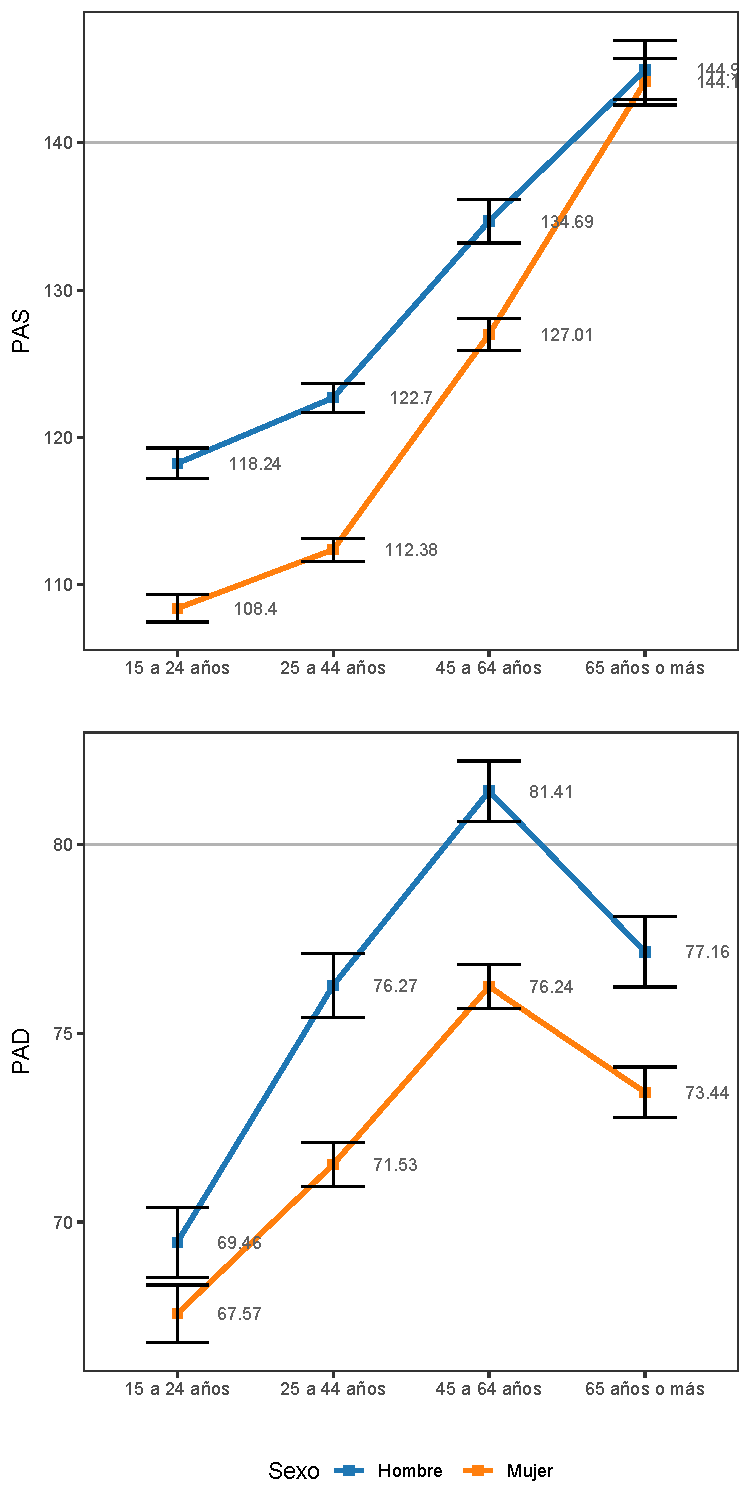
\includegraphics[scale = .55]{img/figura1.pdf}
  \caption{Promedio de presión arterial sistólica y diastólica según el grupo de edad diferenciado por sexo.}
\end{figure}
%%%%%%%%%%%%%%%%%%%%%%%%%%%%%%%%%%%%%%%%%%%%%%%%%%%%%%%%%%%%%%%%%%%%%%%
%%%%%%%%%%%%%%%%%%%%%%%%%%%%

Considerando esta distribuicón de los datos, se estimó la prevalencia de hipertensión. En primer lugar, se observa la distribución de la prevalencia por grupo sociodemográfico. En el grupo de hombres, a el 45\% se le consideraría hipertenso, mientras que en el grupo de mujeres, sólo el 32\% padecería hipertensión. Observamos que, además, la prevalencia aumenta de proporción según categoría de edad. La prevalencia general de la población es de un poco más de un tercio (casi dos quintos), se supera el 40\% de prevalencia a partir de los 45 años y para el próximo tramo etario esta proporción aumenta en 20 puntos porcentuales. En cuanto a distribución geográfica, se observa que en la zona centro sur y sur se alcanza una proporción de hipertensos mayor al promedio nacional, el patrón de prevalencia parece señalar que al aproximarnos al sur del país la hipertensión aumentaría. Por lo demás, las personas que no trabajan tienen una cantidad ligeramente mayor de hipertensos entre ellos, esta comparación es significativa, pero seguramente se debe la población joven laboralmente inactiva es recortada a partir de los 15, edad desde la que está permitido trabajar, de este modo la población laboralmente inactiva considera a la población de retirados, pero solo a una parte de jóvenes inactivos. En suma, ya podemos observar cómo la relación entre edad e hipertensión se ve reforzada.

%%%%%% TABLA N %%%%%%%%%%%%%%%%%%%%%%%%%%%%%%%%%%%%%%%%%%%%%%%%%%%%%%%%
%%%%%%%%%%%%%%%%%%%%%%%%%%%%%%%%%%%%%%%%%%%%%%%%%%%%%%%%%%%%%%%%%%%%%%%
\begin{table}[]
\caption{\small Prevalencia de hipertensión por estratificación y grupo sociodemográfico}
    \centering
    \small
    
    \begin{tabular}{lccc}
\toprule
\textbf{hipertensión} & \textbf{No}, N = 3,503 & \textbf{Sí}, N = 2,013 & valor-p \\ 
\midrule
Sexo &  &  & <0.001 \\ 
\-\hspace{5mm} \tiny Hombre & 1,111 (55\%) & 906 (45\%) &  \\ 
\-\hspace{5mm} \tiny Mujer & 2,392 (68\%) & 1,107 (32\%) &  \\ 
Categoría de edad &  &  & <0.001 \\ 
\-\hspace{5mm} \tiny 15 a 24 años & 668 (92\%) & 60 (8.2\%) &  \\ 
\-\hspace{5mm} \tiny 25 a 44 años & 1,224 (78\%) & 347 (22\%) &  \\ 
\-\hspace{5mm} \tiny 45 a 64 años & 1,047 (56\%) & 810 (44\%) &  \\ 
\-\hspace{5mm} \tiny 65 años o más & 564 (41\%) & 796 (59\%) &  \\ 
Zona &  &  & <0.001 \\ 
\-\hspace{5mm} \tiny Norte & 788 (69\%) & 353 (31\%) &  \\ 
\-\hspace{5mm} \tiny Metropolitana & 558 (67\%) & 273 (33\%) &  \\ 
\-\hspace{5mm} \tiny Centro-Sur & 1,287 (61\%) & 817 (39\%) &  \\ 
\-\hspace{5mm} \tiny Sur & 870 (60\%) & 570 (40\%) &  \\ 
Trabajo &  &  & 0.006 \\ 
\-\hspace{5mm} \tiny Sí & 1,337 (66\%) & 693 (34\%) &  \\ 
\-\hspace{5mm} \tiny No & 2,166 (62\%) & 1,320 (38\%) &  \\ 
 \bottomrule
\end{tabular}
    \vspace{1ex}
    
    {\raggedright \small \textbf{Fuente:} Elaborado a partir de los datos de la Encuesta Nacional de Salud 2017 \par}
\end{table}
%%%%%%%%%%%%%%%%%%%%%%%%%%%%%%%%%%%%%%%%%%%%%%%%%%%%%%%%%%%%%%%%%%%%%%%
%%%%%%%%%%%%%%%%%%%%%%%%%%%%%%%%%%%%%%%%%%%%%%%%%%%%%%%%%%%%%%%%%%%%%%%

%%%%%% TABLA N %%%%%%%%%%%%%%%%%%%%%%%%%%%%%%%%%%%%%%%%%%%%%%%%%%%%%%%%
%%%%%%%%%%%%%%%%%%%%%%%%%%%%%%%%%%%%%%%%%%%%%%%%%%%%%%%%%%%%%%%%%%%%%%%
\begin{table}[]
\caption{\small Prevalencia de hipertensión por factor de riesgo}
    \centering
    \tiny

\captionsetup[table]{labelformat=empty,skip=1pt}
\begin{tabular}{lccc}
\toprule
\textbf{hipertensión} & \textbf{No}, N = 3,503 & \textbf{Sí}, N = 2,013 & valor-p \\ 
\midrule
Categoría de IMC &  &  & <0.001 \\ 
\-\hspace{5mm} \tiny Peso insuficiente & 38 (73\%) & 14 (27\%) &  \\ 
\-\hspace{5mm} \tiny Normopeso & 975 (76\%) & 312 (24\%) &  \\ 
\-\hspace{5mm} \tiny Sobrepeso & 1,334 (64\%) & 752 (36\%) &  \\ 
\-\hspace{5mm} \tiny Obesidad & 1,139 (55\%) & 915 (45\%) &  \\ 
Diabetes &  &  & <0.001 \\ 
\-\hspace{5mm} \tiny No & 3,062 (66\%) & 1,588 (34\%) &  \\ 
\-\hspace{5mm} \tiny Sí & 409 (50\%) & 406 (50\%) &  \\ 
Fuma &  &  & <0.001 \\ 
\-\hspace{5mm} \tiny No & 2,426 (61\%) & 1,530 (39\%) &  \\ 
\-\hspace{5mm} \tiny Sí & 1,077 (69\%) & 483 (31\%) &  \\ 
Hipercolesterolemia &  &  & <0.001 \\ 
\-\hspace{5mm} \tiny No & 1,802 (69\%) & 808 (31\%) &  \\ 
\-\hspace{5mm} \tiny Sí & 564 (52\%) & 526 (48\%) &  \\ 
Depresión &  &  & 0.068 \\ 
\-\hspace{5mm} \tiny No & 2,683 (63\%) & 1,584 (37\%) &  \\ 
\-\hspace{5mm} \tiny Sí & 789 (66\%) & 411 (34\%) &  \\ 
 \bottomrule
\end{tabular}

    {\raggedright \small \textbf{Fuente:} Elaborado a partir de los datos de la Encuesta Nacional de Salud 2017 \par}
\end{table}
%%%%%%%%%%%%%%%%%%%%%%%%%%%%%%%%%%%%%%%%%%%%%%%%%%%%%%%%%%%%%%%%%%%%%%%
%%%%%%%%%%%%%%%%%%%%%%%%%%%%%%%%%%%%%%%%%%%%%%%%%%%%%%%%%%%%%%%%%%%%%%%

Luego, observamos la prevalencia de hipertensión según las clasificaciones de factores de riesgo resumida en la Tabla 4. Al ajustar un test de $\chi^2$ observamos que todas las relaciones son significativas menos la relación con la depresión, por lo que queda descartada como factor de riesgo relevante. Es importante notar que para todos los factores de riesgo la prevalencia de hipertensión alcanza la mitad del grupo afectado con la condición, en el caso de la diabetes, la prevalencia de HTA en población diabética es del 50\% exacto. Esto se cumple para todos los casos, menos para la población de fumadores. 

Hasta el momento hemos revisado por medio de test de $\chi^2$ y test t para medias las relaciones y dependencia entre los factores de riesgo e hipertensión, asentando ideas sobre las posbles asociaciones entre los factores indicados en la literatura. La mayoría, a excepción de la depresión, resultaron en relaciones de un alto grado de significancia ($p <0.001$). En particular, mientras que las categorías de menor riesgo mantienen niveles de prevalencia inferiores o iguales al promedio nacional ($\frac{1}{3}$), la proporción de hipertensos en los grupos que refieren a factores de riesgo tiende a ser de la mitad, excluyendo el caso de los fumadores, cifra que es alarmante. Con el propósito de acercarnos a un lenguaje de propensión y riesgo de desarrollo de patologías, se estimaron \textit{Odds Ratio} con el interés de comparar la propensión de las últimas categorías de las variables teniendo como referencia los odds de las primeras categorías que parecían no verse afectadas.

Al observar la tabla 5, los resultados se condicen con lo discutido. A medida de que aumenta la edad, la persona es más propensa a desarrollar HTA. Se estima que a partir de los 65 años, se es 15 veces más propenso que la categoría mpas joven de desarrollar hipertensión. Incluso antes de llegar a la tercera edad, una persona que entra en la categoría de los 25 años es 3 veces más propensa y la diferencia con las categorías subsiguientes, como es posible observar, es creciente. Por lo demás, la predisposición a desarrollar HTA padeciendo diabetes e hipercolesterolemia dobla la propensión de contraer hipertensión sin estas condiciones. Por lo demás, en el caso de fumadores documenta un odd menor a 1, de forma significativa, esto significaría que la propensión de desarrollar hipertensión es menor que la de no desarrollarla todavía en comparación a la propensión de un no fumador, con respecto a este hallazgo, cabe comentar que sabemos que fumar puede causar un aumento en la presión, pero la evidencia no señala que sea responsable de la conidición crónica de HTA, pues la literatura parece asociar el tabaquismo a los accidentes cardiacos, por lo que la cruzada en contra del consumo de cigarrillos podría ir en una línea paralela a la de la hipertensión, del mismo modo con los malos hábitos alimenticios y la preponderancia de obesidad en la población en general.

\begin{table}[]
\caption{\small Odds Ratio Factores de Riesgo de HTA}
    \centering
    \small
\begin{tabular}{lrcr}
\toprule
  & OR & IC95\% & valor-p\\
\midrule
Categoría de edad\\
\-\hspace{5mm} \tiny  15 a 24 años (ref) & 1.00 & & <0.001\\
\-\hspace{5mm} \tiny  25 a 44 años & 3.16 & [2.36-4.22] & <0.001\\
\-\hspace{5mm} \tiny  45 a 64 años & 8.61 & [6.51-11.39] & <0.001\\
\-\hspace{5mm} \tiny  65 años o más & 15.71 & 11.81-20.90] & <0.001\\
\addlinespace
Categoría de IMC\\
\-\hspace{5mm} \tiny  Peso insuficiente (ref) & 1.00 &  & 0.66\\
\-\hspace{5mm} \tiny  Normopeso & 0.87 & [0.46-1.62] & 0.18\\
\-\hspace{5mm} \tiny  Sobrepeso & 1.53 & [0.82-2.84] & 0.01\\
\-\hspace{5mm} \tiny  Obesidad & 2.18 & [1.17-4.05] & <0.001\\
\addlinespace
Hombre = 1 & 1.76 & [1.57-1.97] & <0.001\\
Diabetes & 1.91 & [1.65-2.22] & <0.001\\
\addlinespace
Fuma & 0.71 & [0.63-0.81] & <0.001\\
\addlinespace
Hipercolesterolemia & 2.08 & [1.80-2.40] & <0.001\\
\bottomrule
\end{tabular}
    \vspace{1ex}
    
    {\raggedright \small \textbf{Fuente:} Elaborado a partir de los datos de la Encuesta Nacional de Salud 2017 \par}
\end{table}

%%%%%%%%%%%%%%%%%%%%%%%%%%%%%%%%%%%%%%%%%%%%%%%%%%%%%%%%%%%%%%%%%%%%%%%
%%%%%%%%%%%%%%%%%%%%%%%%%%%%%%%%%%%%%%%%%%%%%%%%%%%%%%%%%%%%%%%%%%%%%%%

\section{Conclusión y Discusión}

El presente estudio tuvo el objetivo de estimar la prevalencia hipertensión arterial y su asociación con otras enfermedades. Hallamos que cerca de dos quintos de la muestra podría ser diagnosticada con hipertensión, sin embargo, sólo un 12\% reconoce tener un diagnóstico de hipertensión y un 22\% declara haber sido advertido por sus niveles de presión arterial en alguna oportunidad, lo que delataría que esta afección sigue siendo un \textit{asunto desatendido}. 

En cuanto a los factores de riesgo, se encontró que dentro de los grupos que manifestaban estas condiciones, cerca de la mitad eran hipertensas, con excepción del grupo de fumadores. 

El hallazgo más importante consiste en las implicancias del envejecimiento en la propensión a desarrollar HTA, no es posible comprender el efecto de la hipertensión en los factores sociodemográficos como el género si no se observa en función de la edad, es así, como los hombres y las mujeres no parecen, a priori, tener diferencias substanciales en cuanto a presión arterial, esta diferencia sólo se hace evidente a la hora de considerar cómo se comporta la hipertensión en hombres y mujeres.

Muchos de los hallazgos coinciden con lo revisado en la literatura, a excepción de ciertos factores de riesgo que no tienen una asociación directa con factores etiológicos sino, más bien, con las complicaciones asociadas, como es el caso del tabaco y la masa corporal, la cual resultó ser poco significativa en el análisis de comparación de \textit{odds}. Asuntos de la literatura reciente, como factores emocionales y nuevos casos de presión diastólica elevada en población jóven, no pudo ser constatada. En suma, se reitera la importancia de la investigación como generador de conocimientos comunes y populares sobre cómo y cuánto consultar nuestro estado de salud con un médico. Gracias a la investigación biomédica, es de conocimiento popular monitoriar la presión arterial después de los 40 años de edad. Se espera, entonces, que la generación de evidencia sigua en curso y, en sí misma, aporte a información a las deciciones de las personas.




\section{Referencias Bibliográficas}

\tiny
\begin{hangparas}{.25in}{1}

Álvarez-Ochoa, R., Pinguil-Yugsi, M., \& Cordero-Cordero, G. (2019). Factores de riesgo de hipertensión arterial en adolescentes Risk factors for arterial hypertension in adolescents. Revista Científica y Tecnológica UPSE, 5(2), 111-118. Recuperado de

Buford, T. W. (2016). Hypertension and aging. Ageing research reviews, 26, 96-111.

Ferrier, K. E., Muhlmann, M. H., Baguet, J. P., Cameron, J. D., Jennings, G. L., Dart, A. M., \& Kingwell, B. A. (2002). Intensive cholesterol reduction lowers blood pressure and large artery stiffness in isolated systolic hypertension. Journal of the American College of Cardiology, 39(6), 1020-1025.

Flynn, J. T. (2009). Hypertension in the young: epidemiology, sequelae and therapy. Nephrology Dialysis Transplantation, 24(2), 370-375.

Grigore, D., Ojeda, N. B., \& Alexander, B. T. (2008). Sex differences in the fetal programming of hypertension. Gender medicine, 5, S121-S132.

Lancet, T. (2007). Hypertension: uncontrolled and conquering the world.

Mancia, G., Fagard, R., Narkiewicz, K., Redón, J., Zanchetti, A., Böhm, M., ... \& Zannad, F. (2013). 2013 ESH/ESC Guidelines for themanagement of arterial hypertension The Task Force for the management ofarterial hypertension of the European Society ofHypertension (ESH) and of the European Society of Cardiology (ESC). Journal of hypertension, 31(7), 1281-1357.

Margozzini, P., \& Passi, Á. (2018). Encuesta Nacional de Salud, ENS 2016-2017: un aporte a la planificación sanitaria y políticas públicas en Chile. ars medica revista de ciencias médicas, 43(1), 30-34.

Medicna Ambulatoria. (20201). Retrieved 11 December 2021, from http://publicacionesmedicina.uc.cl/MedAmb/Hipertensionarterial.html % no citado aun

Messerli, F. H., Williams, B., \& Ritz, E. (2007). Essential hypertension. The Lancet, 370(9587), 591-603.

Organización Mundial de la Salud [OMS]. (2021). Retrieved 11 December 2021, from https://www.who.int/es/news-room/fact-sheets/detail/hypertension

Petermann, F., Durán, E., Labraña, A. M., Martínez, M. A., Leiva, A. M., Garrido-Méndez, A., ... \& Celis-Morales, C. (2017). Factores de riesgo asociados al desarrollo de hipertensión arterial en Chile. Revista médica de Chile, 145(8), 996-1004.

Petermann-Rocha, F., Sillars, A., Brown, R., Sweeney, L., Troncoso, C., García-Hermoso, A., . . . Celis-Morales, C. (2019). Sociodemographic patterns of urine sodium excretion and its association with hypertension in Chile: A cross-sectional analysis. Public Health Nutrition, 22(11), 2012-2021. doi:10.1017/S1368980018003889

Petrie, J. R., Guzik, T. J., \& Touyz, R. M. (2018). Diabetes, hypertension, and cardiovascular disease: clinical insights and vascular mechanisms. Canadian Journal of Cardiology, 34(5), 575-584.

Riveros, A., Ceballos, G., Laguna, R., \& Sánchez-Sosa, J. J. (2005). El manejo psicológico de la hipertensión esencial: efectos de una intervención cognitivo-conductual. Revista Latinoamericana de Psicología, 37(3), 493-507.

Saval (2011). “Hay una relación muy peligrosa entre la mujer fumadora y hormonas”. Retrieved 11 December 2021, from https://www.savalnet.cl/mundo-medico/entrevistas/21555.html

Tagle, R. (2018). Diagnóstico de hipertensión arterial. Revista Médica Clínica Las Condes, 29(1), 12-20.

Tapia, M. L., \& Labiano, L. M. (2004). Factores emocionales e hipertensión esencial. Terapia Psicológica, 22(2), 103-109.

Tibazarwa, K. B., \& Damasceno, A. A. (2014). Hypertension in developing countries. Canadian Journal of Cardiology, 30(5), 527-533. 

Virdis, A., Giannarelli, C., Fritsch Neves, M., Taddei, S., \& Ghiadoni, L. (2010). Cigarette smoking and hypertension. Current pharmaceutical design, 16(23), 2518-2525.


\end{hangparas}

\end{document}
